%----------------------------------------------------------
\def\notedate{2021.11.22}
\def\currentauthor{Крехтунова Д.Д. (РК6-73Б)}
%----------------------------------------------------------
\notestatement{rndhpcedt}{Первичный обзор литературы КП МО}

%---------------------------------------------------------
\subsubsection{Ассоциативные массивы}

Ассоциативный массив – это массив, в котором обращение к значению осуществляется по ключу.

При этом в качестве ключа используется не индекс, а строка, задаваемая программистом. Таким образом представить ассоциативный массив можно как набор пар «ключ-значение». При этом каждое значение связано с определённым ключом.

Поддержка ассоциативных массивов есть во многих интерпретируемых языках программирования высокого уровня, таких, как Perl, PHP, Python, Ruby, Tcl, JavaScript и других.

\paragraph{Реализации ассоциативного массива}
\

Простейший способ хранения ассоциативных массивов – список пар (ключ, значение), где Ключ определяет индекс элемента, а Значение – значение элемента с этим индексом.

Но наиболее популярными являются реализации, основанные на различных деревьях поиска. 
Так, например, в стандартной библиотеке STL языка C++ контейнер map реализован на основе красно-чёрного дерева. В языках Java, Ruby, Tcl, Python используется один из вариантов хеш-таблицы. Есть и другие реализации.

Операции с деревом работают быстрее. При реализации списком все функции требуют O(n) действий, где n — размер структуры. Операции с деревом же работают за O(h), где h — максимальная глубина дерева.

Данные в дереве хранятся в его вершинах. В программах вершины дерева обычно представляют структурой, хранящей данные и две ссылки на левого и правого сына. 

\begin{figure}[h]
	\centering
	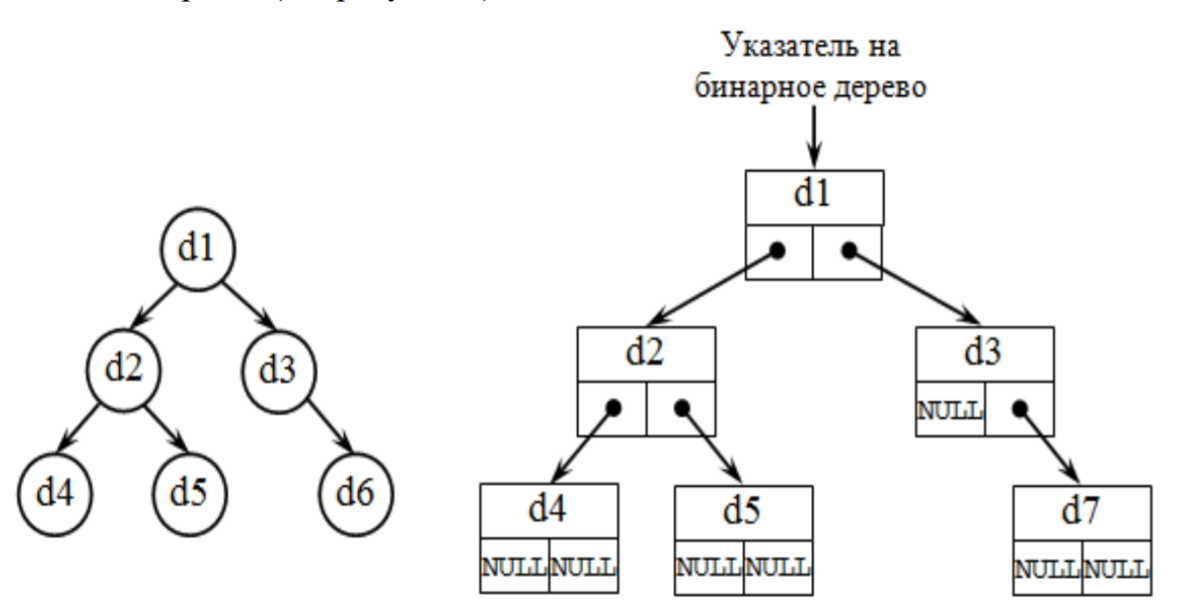
\includegraphics[width=0.6\textwidth]{ResearchNotes/rndhpc_not_edt_2021_11_22/bin_tree.png}
	\caption{Пример представления бинарного дерева} 
\end{figure}

\subsubsection{TnT: набор библиотек для web-визуализации деревьев и аннотаций на основе трассировок \cite{Pignatelli2016}}

В статье представлен набор библиотек, предназначенных для web визуализации деревьев и трассировок.

В статье говорится в первую очередь о визуализации биологических данных в веб-приложениях. Но представленные библиотеки не имеют узкой направленности и могут использоваться для разных целей.

Библиотеки TnT (Trees and Tracks) предназначены для создания настраиваемых, динамических и интерактивных визуализаций деревьев и аннотаций на основе треков. 

Библиотеки написаны на Javascript с использованием библиотеки D3, которая сама по себе является мощным инструментом визуализации данных. Она использует стандарты масштабируемой векторной графики (SVG), HTML и CSS.

Ниже приведено краткое описание библиотек TnT, непосредственно связанных с визуализацией деревьев:

\begin{itemize}
	\item \textit{TnT Tree}
	
	Эта библиотека построена на основе кластерного расположения D3 (D3 cluster layout) и позволяет создавать динамические и интерактивные деревья. Он состоит из нескольких настраиваемых элементов: макета, определяющего общую форму дерева, узлов дерева в которых можно изменять форму, размер и цвет, ярлыков, состоящих из текста или изображений и данных для загрузки объектов Javascript или строк newick / nhx.2.2 TnT Tree Node.
	
	PhyloCanvas - аналогичный проект, предлагающий средства для визуализации деревьев. В качестве основной технологии в нем используется Canvas. Но библиотеки TnT более универсальны и поддерживают интеграцию с другими библиотеками. Документацию и примеры для TnT Tree можно найти по ссылке http://tntvis.github.io/tnt.tree/.
	
	\item \textit{TnT Tree Node}	
	
	Эта библиотека предоставляет методы для управления деревом на уровне данных и используется TnT Tree, хотя также может использоваться и независимо. Методы, включенные в TnT Tree Node, варьируются от вычисления наименьшего общего предка набора узлов до извлечения поддеревьев. Документацию для этой библиотеки можно найти как часть документации библиотеки TnT Tree.
\end{itemize}

\subsubsection{Empress: обеспечение интерактивного и исследовательского анализа многомерных наборов данных на основе деревьев \cite{Cantrell2021}}

Здесь представлен интерактивный веб-инструмент EMPress для визуализации деревьев в контексте микробиома, метаболома и других областей. EMPress предоставляет широкие функциональные возможности, такие как анимация объектов, наряду со стандартными функциями визуализации дерева.

EMPress реализован в виде подключаемого модуля QIIME 2 (или отдельной программы Python, которую можно использовать вне QIIME 2), способной создавать HTML-документы с автономным пользовательским интерфейсом визуализации. Кодовая база состоит из компонента Python и компонента JavaScript. Кодовая база Python отвечает за проверку данных, предварительную обработку, фильтрацию и форматирование. Взаимодействие с пользователем, рендеринг и генерация рисунков обрабатываются базой кода JavaScript. 

Кодовая база Python EMPress использует такие модули, как NumPy, SciPy, Pandas, Click, Jinja2, scikit-bio, формат BIOM и EMPeror. 

В кодовой базе JavaScript используются Chroma.js, FileSaver.js, glMatrix, jQuery, Require.js, Spectrum, и Underscore.js. 

\subsubsection{Treemap: инструмент визуализации иерархических структур \cite{Jadeja2020}}

В статье представлена интерактивная версия Treemap.

В теории графов дерево - это особый тип графа, который связан и ацикличен. Обычно деревья представляются визуально с помощью диаграмм узлов и связей (древовидных диаграмм). В деревьях ребра присутствуют только между соседними слоями, и, следовательно, деревья наиболее подходят для представления иерархических данных (где элементы представлены как находящиеся «ниже», «выше» или «на одном уровне» друг с другом).

Treemap - это метод визуализации иерархических структур. Используя этот метод, можно отобразить дерево с миллионами узлов в ограниченном пространстве. Основная идея, лежащая в основе этого метода визуализации, состоит в том, чтобы выделиять прямоугольники для родительских узлов, а для дочерних узлов блоки (прямоугольники) в соответствующем родительском прямоугольнике. 

Интерфейс создавался с использованием html / css с jQuery для обработки событий, связанных с кликами.Входными данными для интерфейса является дерево родительских указателей (parent pointer tree - структура данных N-арного дерева, в которой каждый узел имеет указатель на свой родительский узел, но не указывает на дочерние узлы). 

\subsubsection{DoubleRecViz: веб-инструмент для визуализации согласования деревьев транскриптов и генов \cite{Kuitche2021}}

В статье представлен веб-инструмент для визуализации согласований между филогенетическими деревьями (деревья, отражающее эволюционные взаимосвязи между различными видами, имеющими общего предка).

В статье описан формат DoubleRecViz, основанный на формате phyloXML (XML, предназначенный для описания филогенетических деревьев и связанных с ними данных). 

DoubleRecViz написан на Python и использует библиотеку Dash, которая предоставляет функции динамической визуализации веб-данных.
Dash является связкой Flask, React.Js, HTML и CSS.

Приложения на Dash — веб-серверы, которые запускают Flask и связывают пакеты JSON через HTTP-запросы. Интерфейс Dash формирует компоненты, используя React.js.

Компоненты Dash — это классы Python, которые кодируют свойства и значения конкретного компонента React и упорядочиваются как JSON. 

Полный набор HTML-тегов также обрабатывается с помощью React, а их классы Python доступны через библиотеку. CSS и стили по умолчанию хранятся вне базовой библиотеки, чтобы сохранить принцип модульности и независимого управления версиями.

%----------------------------------------------------------
% Атрибуты задачи
\noteattributes{}
%----------------------------------------------------------

